\documentclass[]{book}
\usepackage{lmodern}
\usepackage{amssymb,amsmath}
\usepackage{ifxetex,ifluatex}
\usepackage{fixltx2e} % provides \textsubscript
\ifnum 0\ifxetex 1\fi\ifluatex 1\fi=0 % if pdftex
  \usepackage[T1]{fontenc}
  \usepackage[utf8]{inputenc}
\else % if luatex or xelatex
  \ifxetex
    \usepackage{mathspec}
  \else
    \usepackage{fontspec}
  \fi
  \defaultfontfeatures{Ligatures=TeX,Scale=MatchLowercase}
\fi
% use upquote if available, for straight quotes in verbatim environments
\IfFileExists{upquote.sty}{\usepackage{upquote}}{}
% use microtype if available
\IfFileExists{microtype.sty}{%
\usepackage{microtype}
\UseMicrotypeSet[protrusion]{basicmath} % disable protrusion for tt fonts
}{}
\usepackage[margin=1in]{geometry}
\usepackage{hyperref}
\hypersetup{unicode=true,
            pdftitle={Sociospatial Data Science},
            pdfauthor={Christopher Prener, Ph.D.},
            pdfborder={0 0 0},
            breaklinks=true}
\urlstyle{same}  % don't use monospace font for urls
\usepackage{natbib}
\bibliographystyle{apalike}
\usepackage{color}
\usepackage{fancyvrb}
\newcommand{\VerbBar}{|}
\newcommand{\VERB}{\Verb[commandchars=\\\{\}]}
\DefineVerbatimEnvironment{Highlighting}{Verbatim}{commandchars=\\\{\}}
% Add ',fontsize=\small' for more characters per line
\usepackage{framed}
\definecolor{shadecolor}{RGB}{248,248,248}
\newenvironment{Shaded}{\begin{snugshade}}{\end{snugshade}}
\newcommand{\KeywordTok}[1]{\textcolor[rgb]{0.13,0.29,0.53}{\textbf{{#1}}}}
\newcommand{\DataTypeTok}[1]{\textcolor[rgb]{0.13,0.29,0.53}{{#1}}}
\newcommand{\DecValTok}[1]{\textcolor[rgb]{0.00,0.00,0.81}{{#1}}}
\newcommand{\BaseNTok}[1]{\textcolor[rgb]{0.00,0.00,0.81}{{#1}}}
\newcommand{\FloatTok}[1]{\textcolor[rgb]{0.00,0.00,0.81}{{#1}}}
\newcommand{\ConstantTok}[1]{\textcolor[rgb]{0.00,0.00,0.00}{{#1}}}
\newcommand{\CharTok}[1]{\textcolor[rgb]{0.31,0.60,0.02}{{#1}}}
\newcommand{\SpecialCharTok}[1]{\textcolor[rgb]{0.00,0.00,0.00}{{#1}}}
\newcommand{\StringTok}[1]{\textcolor[rgb]{0.31,0.60,0.02}{{#1}}}
\newcommand{\VerbatimStringTok}[1]{\textcolor[rgb]{0.31,0.60,0.02}{{#1}}}
\newcommand{\SpecialStringTok}[1]{\textcolor[rgb]{0.31,0.60,0.02}{{#1}}}
\newcommand{\ImportTok}[1]{{#1}}
\newcommand{\CommentTok}[1]{\textcolor[rgb]{0.56,0.35,0.01}{\textit{{#1}}}}
\newcommand{\DocumentationTok}[1]{\textcolor[rgb]{0.56,0.35,0.01}{\textbf{\textit{{#1}}}}}
\newcommand{\AnnotationTok}[1]{\textcolor[rgb]{0.56,0.35,0.01}{\textbf{\textit{{#1}}}}}
\newcommand{\CommentVarTok}[1]{\textcolor[rgb]{0.56,0.35,0.01}{\textbf{\textit{{#1}}}}}
\newcommand{\OtherTok}[1]{\textcolor[rgb]{0.56,0.35,0.01}{{#1}}}
\newcommand{\FunctionTok}[1]{\textcolor[rgb]{0.00,0.00,0.00}{{#1}}}
\newcommand{\VariableTok}[1]{\textcolor[rgb]{0.00,0.00,0.00}{{#1}}}
\newcommand{\ControlFlowTok}[1]{\textcolor[rgb]{0.13,0.29,0.53}{\textbf{{#1}}}}
\newcommand{\OperatorTok}[1]{\textcolor[rgb]{0.81,0.36,0.00}{\textbf{{#1}}}}
\newcommand{\BuiltInTok}[1]{{#1}}
\newcommand{\ExtensionTok}[1]{{#1}}
\newcommand{\PreprocessorTok}[1]{\textcolor[rgb]{0.56,0.35,0.01}{\textit{{#1}}}}
\newcommand{\AttributeTok}[1]{\textcolor[rgb]{0.77,0.63,0.00}{{#1}}}
\newcommand{\RegionMarkerTok}[1]{{#1}}
\newcommand{\InformationTok}[1]{\textcolor[rgb]{0.56,0.35,0.01}{\textbf{\textit{{#1}}}}}
\newcommand{\WarningTok}[1]{\textcolor[rgb]{0.56,0.35,0.01}{\textbf{\textit{{#1}}}}}
\newcommand{\AlertTok}[1]{\textcolor[rgb]{0.94,0.16,0.16}{{#1}}}
\newcommand{\ErrorTok}[1]{\textcolor[rgb]{0.64,0.00,0.00}{\textbf{{#1}}}}
\newcommand{\NormalTok}[1]{{#1}}
\usepackage{longtable,booktabs}
\usepackage{graphicx,grffile}
\makeatletter
\def\maxwidth{\ifdim\Gin@nat@width>\linewidth\linewidth\else\Gin@nat@width\fi}
\def\maxheight{\ifdim\Gin@nat@height>\textheight\textheight\else\Gin@nat@height\fi}
\makeatother
% Scale images if necessary, so that they will not overflow the page
% margins by default, and it is still possible to overwrite the defaults
% using explicit options in \includegraphics[width, height, ...]{}
\setkeys{Gin}{width=\maxwidth,height=\maxheight,keepaspectratio}
\IfFileExists{parskip.sty}{%
\usepackage{parskip}
}{% else
\setlength{\parindent}{0pt}
\setlength{\parskip}{6pt plus 2pt minus 1pt}
}
\setlength{\emergencystretch}{3em}  % prevent overfull lines
\providecommand{\tightlist}{%
  \setlength{\itemsep}{0pt}\setlength{\parskip}{0pt}}
\setcounter{secnumdepth}{5}
% Redefines (sub)paragraphs to behave more like sections
\ifx\paragraph\undefined\else
\let\oldparagraph\paragraph
\renewcommand{\paragraph}[1]{\oldparagraph{#1}\mbox{}}
\fi
\ifx\subparagraph\undefined\else
\let\oldsubparagraph\subparagraph
\renewcommand{\subparagraph}[1]{\oldsubparagraph{#1}\mbox{}}
\fi

%%% Use protect on footnotes to avoid problems with footnotes in titles
\let\rmarkdownfootnote\footnote%
\def\footnote{\protect\rmarkdownfootnote}

%%% Change title format to be more compact
\usepackage{titling}

% Create subtitle command for use in maketitle
\newcommand{\subtitle}[1]{
  \posttitle{
    \begin{center}\large#1\end{center}
    }
}

\setlength{\droptitle}{-2em}
  \title{Sociospatial Data Science}
  \pretitle{\vspace{\droptitle}\centering\huge}
  \posttitle{\par}
  \author{Christopher Prener, Ph.D.}
  \preauthor{\centering\large\emph}
  \postauthor{\par}
  \predate{\centering\large\emph}
  \postdate{\par}
  \date{2017-09-22}

\usepackage{booktabs}
\usepackage{amsthm}
\makeatletter
\def\thm@space@setup{%
  \thm@preskip=8pt plus 2pt minus 4pt
  \thm@postskip=\thm@preskip
}
\makeatother

\usepackage{amsthm}
\newtheorem{theorem}{Theorem}[chapter]
\newtheorem{lemma}{Lemma}[chapter]
\theoremstyle{definition}
\newtheorem{definition}{Definition}[chapter]
\newtheorem{corollary}{Corollary}[chapter]
\newtheorem{proposition}{Proposition}[chapter]
\theoremstyle{definition}
\newtheorem{example}{Example}[chapter]
\theoremstyle{definition}
\newtheorem{exercise}{Exercise}[chapter]
\theoremstyle{remark}
\newtheorem*{remark}{Remark}
\newtheorem*{solution}{Solution}
\begin{document}
\maketitle

{
\setcounter{tocdepth}{1}
\tableofcontents
}
\chapter*{Preface}\label{preface}
\addcontentsline{toc}{chapter}{Preface}

\begin{center}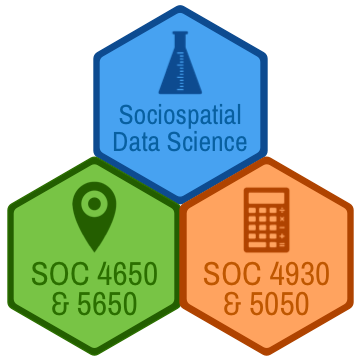
\includegraphics[width=0.4\linewidth]{images/SSDSBookBanner} \end{center}

This text is a companion text for both of my research methods courses at
\href{https://slu.edu}{Saint Louis University}:

\begin{itemize}
\tightlist
\item
  \href{https://slu-soc5650.github.io}{SOC 4650/5650 - Introduction to
  Geographic Information Science}
\item
  \href{https://slu-soc5050.github.io}{SOC 4930/5050 - Quantitative
  Analysis: Applied Inferential Statistics}
\end{itemize}

The goal of the text is to create a reference for the intangible, subtle
or disparate skills and ideas that contribute to being a successful
\emph{computational} social scientist. In writing this text, I draw
inspiration from the work of Donald Knuth.\footnote{\href{https://en.wikipedia.org/wiki/Donald_Knuth}{Donald
  Knuth} is the developer of
  \href{https://en.wikipedia.org/wiki/TeX}{TeX}, a computer typesetting
  system that is widely used today for scientific publishing in the form
  of \href{https://en.wikipedia.org/wiki/LaTeX}{LaTeX}. He also
  established the concept of
  \href{https://en.wikipedia.org/wiki/Literate_programming}{literate
  programming}, which forms the basis of some of the practices we follow
  with \texttt{R}.} Knuth has discussed his experiences in designing new
software languages, nothing that the developer of a new language

\begin{quote}
\ldots{}must not only be the implementer and the first large-scale user;
the designer should also write the first user manual\ldots{} If I had
not participated fully in all these activities, literally hundreds of
improvements would never have been made, because I would never have
thought of them or perceived why they were important\ldots{}
\end{quote}

While there is nothing particularly new about what I am writing here,
and I am certainly not developing a new language for computing, the goal
of this text remains similar to Knuth's experience. By distilling some
of key elements for making a successful transition to being a
\emph{professional developer} of knowledge rather than a \emph{casual
consumer}, I hope to both improve the course experience itself and also
create an environment that fosters a successful learning experience for
you.

In both classes, the course names are deceptive. We are not only
concerned with statistical work or mapping. Rather, we are more
fundamentally concerned with research methods. In particular, we are
concerned with \emph{high quality} research methods and the
\emph{process} of conducting research. We therefore focus on a
combination of mental habits and technical practices that make you a
successful researcher. Some of the skills and techniques that we will
discuss this semester are not taught as often in graduate programs, let
along undergraduate programs. Instead, they are often the products of
``learning the hard way''. These ``habits of mind and habits of method''
are broadly applicable across methodologies and disciplines.

\section*{License}\label{license}
\addcontentsline{toc}{section}{License}

Copyright © 2016-2017 \href{https://chris-prener.github.io}{Christopher
G. Prener}

This work is licensed under a Creative Commons Attribution 4.0
International License.

\chapter{Introduction}\label{intro}

The first part of this text is designed to help get you oriented to
coursework in computational social science. Both
\href{https://slu-soc5650.github.io}{Introduction to Geographic
Information Science (SOC 4650/5650)} and
\href{https://slu-soc5050.github.io}{Quantitative Analysis: Applied
Inferential Statistics (SOC 4930/5050)} are focused on building
students' capacities to address social science research questions using
tools that have been the traditional domain of computer and information
scientists. The growth and application of these tools in a variety of
disciplines both inside and outside of the social sciences has come to
be known as data science. Both courses are taught from this perspective,
so that while we focus on social science data, the tools and techniques
are broadly applicable across disciplines.

\section{What is data science?}\label{what-is-data-science}

Given data science's new emergence, its definition remains both
contested and often unclear. For me, there are four key aspects to focus
on when considering what constitutes data science:

\begin{enumerate}
\def\labelenumi{\arabic{enumi}.}
\tightlist
\item
  Statistics
\item
  Programming
\item
  Visualization and Communication
\item
  Substantive Knowledge
\end{enumerate}

I think of this as a ``full stack'' approach to computational research.
You want to be well versed not only the techniques for generating and
analyzing data, but also substantively in the academic literature about
your area of interest as well as ways to communicate your findings with
other researchers and the wider public.

\subsection{Statistics}\label{statistics}

Statistics covers the mathematical techniques that we use to draw
inference from our data. It is the main subject of one my courses,
\href{https://slu-soc5050.github.io}{Quantitative Analysis}. In
\href{https://slu-soc5650.github.io}{Introduction to GIS}, we do not
explicitly cover much in the way of inferential statistics. However, the
course is desinged to prepare you for a next level, Intermediate GIS
course that covers spatial statistics.

\subsection{Programming}\label{programming}

Computer programming is an essential part of data science broadly and
computational social science more specifically. Using a programming
language means that our work can be easily reproduced. This emphasis on
\textbf{reproducibility} is a response to a growing fear in many
disciplines that results are replicable from study to study, which
raises questions about the validity of much of the research work that we
do. Our goal in both courses is to produce research that is as
reproducible as possible.

This book introduces two programming languages -
\href{https://en.wikipedia.org/wiki/R_(programming_language)}{\texttt{R}}
and
\href{https://en.wikipedia.org/wiki/Python_(programming_language)}{Python}.
In \href{https://slu-soc5050.github.io}{Quantitative Analysis}, we will
be focused exclusively on learning \texttt{R} and using it to produce
statistical analyses. In
\href{https://slu-soc5650.github.io}{Introduction to GIS}, we will spend
a lot of time in \texttt{R}, but we will also use some Python to help
pass data from \texttt{R} to ArcGIS, the mapping application we will
use. I will also provide some additional Python lessons to folks who are
interested, but these will not be required for the course.

\subsection{Visualization \&
Communication}\label{visualization-communication}

Visualization is a fundamental aspect of data science work. It is how we
make our results easily digestible and accessible to a wider audience,
many of whom may not be able to interpret statistical output but can
learn from a well-designed scatter plot. In
\href{https://slu-soc5050.github.io}{Quantitative Analysis}, we will
focus on building plots to communicate information about statistical
distributions and the relationships between our variables. In
\href{https://slu-soc5650.github.io}{Introduction to GIS}, we will use
the same fundamental skills to build simple maps in \texttt{R}. We will
extend our emphasis on visualization to ArcGIS, where we will focus on
producing cartographically rich depictions of our data.

Separetely, we will discuss the presentation of statistical data in
tables using \href{https://en.wikipedia.org/wiki/LaTeX}{LaTex} in
\href{https://slu-soc5050.github.io}{Quantitative Analysis} as well as
the producing to conference-style presentations to communicate research
findings. In \href{https://slu-soc5650.github.io}{Introduction to GIS},
we will focus on producing conference-style posters instead. These are
different mediums, but they rely on the same design fundamentals that
are covered in this text.

\subsection{Substantive Knowledge}\label{substantive-knowledge}

Substantive knowledge covers two tangentially related topics: the
ability to work well in groups and the ability to digest and integrate
an academic literature into your own research. Each of these topics
receive some focus in both
\href{https://slu-soc5050.github.io}{Quantitative Analysis} and
\href{https://slu-soc5650.github.io}{Introduction to GIS}. Each class
has some group work associated with the completion with weekly lab
assignments. \href{https://slu-soc5650.github.io}{Introduction to GIS}
also has a group work component associated with the final project. In
each class, students' final projects are focused on a specific content
area that requires at least some background research and knowledge.
Synthesizing this knowledge and integrating it into your final projects
is a key piece of addressing this facet of data science.

\section{How is this book organized?}\label{how-is-this-book-organized}

Like many books about data science, this text follows a number of
standard conventions related to how it is organized and how examples are
given. This section introduces those conventions.

\subsection{Typefaces and Fonts}\label{typefaces-and-fonts}

Technical publications that describe scientific computing processes use
a \texttt{monospaced\ typewriter\ style\ typeface} to refer to commands
(inputs) and results (outputs). In some documents, like lecture slides
and cheat-sheets, I may highlight a command by using a particular color
to increase the visibility of the command name itself.

The \texttt{typewriter\ typeface} is also used to refer to functions
(e.g. \texttt{library()}), filenames (e.g. \texttt{mpg.csv}) or
filepaths (e.g.
\texttt{C:\textbackslash{}Users\textbackslash{}JSmith\textbackslash{}Desktop}).
Finally, we will use the \texttt{typewriter\ typeface} to refer to
GitHub repositories (e.g. \texttt{Core-Documents}, the repository that
contains this file).

Technical publications use \emph{italicized text} to refer to text that
is meant to be replaced. These references will typically appear in a
\texttt{typewriter\ typeface} since they are often part of commands. For
example, \texttt{str(dataFrame)} (with \texttt{dataFrame}
\emph{italicized}) indicates that you should replace the text
\texttt{dataFrame} with the appropriate variable name from your dataset.

These publications also use a sans serif typeface to refer to areas of
the user interface, menu items, and buttons. I cannot replicate that
here because of the publishing software that I use, but you'll notice
this text in course documents. We will therefore use the
\texttt{typewriter\ typeface} in the User Guide to identify these same
features.

Technical documents also use a sans serif or \texttt{typewriter}
typeface to refer to keyboard keys (e.g. \texttt{Crtl+C}) where the plus
sign (\texttt{+}) indicates that you should press multiple keys at the
same time. A sans serif typeface combined with a right facing
triangle-style arrow (\texttt{\textgreater{}}) is used to refer to
actions that require clicking through a hierarchy of menus or windows
(e.g. \texttt{File\ \textgreater{}\ Save}).

\subsection{Data}\label{data}

There are two sets of data that are used in this text, and they are also
used as part of \href{https://slu-soc5050.github.io}{Quantitative
Analysis} and \href{https://slu-soc5650.github.io}{Introduction to GIS}.
Both are available as \texttt{R} packages. The \texttt{testDriveR}
package contains some generic data that are particularly well suited for
exploring statistical topics. The \texttt{stlData} package contains data
that can be mapped at various levels. Both of these packages are
currently available on \href{https://github.com}{GitHub}, and can be
installed using the \texttt{devtools} package:

\begin{Shaded}
\begin{Highlighting}[]
\KeywordTok{install.packages}\NormalTok{(}\StringTok{"devtools"}\NormalTok{)}
\KeywordTok{library}\NormalTok{(devtools)}
\NormalTok{devtools::}\KeywordTok{install_github}\NormalTok{(}\StringTok{"chris-prener/testDriveR"}\NormalTok{)}
\NormalTok{devtools::}\KeywordTok{install_github}\NormalTok{(}\StringTok{"chris-prener/stlData"}\NormalTok{)}
\end{Highlighting}
\end{Shaded}

\subsection{Examples}\label{examples}

Throughout the semester, I will give you examples both in lecture slides
and in an example do-file. Examples in lectures and course documents can
be easily identified by their use of the \texttt{typewriter\ typeface}:

\begin{Shaded}
\begin{Highlighting}[]
\NormalTok{>}\StringTok{ }\KeywordTok{library}\NormalTok{(stlData)}
\NormalTok{>}\StringTok{ }\KeywordTok{str}\NormalTok{(stlLead)}
\StringTok{'data.frame'}\NormalTok{:}\StringTok{   }\DecValTok{106} \NormalTok{obs. of  }\DecValTok{15} \NormalTok{variables:}
\StringTok{ }\ErrorTok{$}\StringTok{ }\NormalTok{geoID         :}\StringTok{ }\NormalTok{num  }\FloatTok{2.95e+10} \FloatTok{2.95e+10} \FloatTok{2.95e+10} \FloatTok{2.95e+10} \FloatTok{2.95e+10} \NormalTok{...}
 \NormalTok{$}\StringTok{ }\NormalTok{tractCE       :}\StringTok{ }\NormalTok{int  }\DecValTok{118100} \DecValTok{117400} \DecValTok{126700} \DecValTok{119102} \DecValTok{126800} \DecValTok{126900} \DecValTok{108100} \DecValTok{127000} \DecValTok{127400} \DecValTok{103700} \NormalTok{...}
 \NormalTok{$}\StringTok{ }\NormalTok{nameLSAD      :}\StringTok{ }\NormalTok{chr  }\StringTok{"Census Tract 1181"} \StringTok{"Census Tract 1174"} \StringTok{"Census Tract 1267"} \StringTok{"Census Tract 1191.02"} \NormalTok{...}
 \NormalTok{$}\StringTok{ }\NormalTok{countTested   :}\StringTok{ }\NormalTok{int  }\DecValTok{345} \DecValTok{871} \DecValTok{458} \DecValTok{182} \DecValTok{486} \DecValTok{1296} \DecValTok{903} \DecValTok{585} \DecValTok{2116} \DecValTok{417} \NormalTok{...}
 \NormalTok{$}\StringTok{ }\NormalTok{pctElevated   :}\StringTok{ }\NormalTok{num  }\FloatTok{9.57} \FloatTok{12.06} \FloatTok{18.12} \FloatTok{2.2} \FloatTok{4.73} \NormalTok{...}
 \NormalTok{$}\StringTok{ }\NormalTok{totalPop      :}\StringTok{ }\NormalTok{int  }\DecValTok{1161} \DecValTok{4307} \DecValTok{1089} \DecValTok{3237} \DecValTok{3490} \DecValTok{4590} \DecValTok{3144} \DecValTok{2052} \DecValTok{5486} \DecValTok{2408} \NormalTok{...}
 \NormalTok{$}\StringTok{ }\NormalTok{totalPop_MOE  :}\StringTok{ }\NormalTok{int  }\DecValTok{192} \DecValTok{447} \DecValTok{199} \DecValTok{309} \DecValTok{231} \DecValTok{826} \DecValTok{464} \DecValTok{273} \DecValTok{516} \DecValTok{274} \NormalTok{...}
 \NormalTok{$}\StringTok{ }\NormalTok{white         :}\StringTok{ }\NormalTok{int  }\DecValTok{414} \DecValTok{2604} \DecValTok{432} \DecValTok{2008} \DecValTok{3026} \DecValTok{148} \DecValTok{108} \DecValTok{304} \DecValTok{1777} \DecValTok{2149} \NormalTok{...}
 \NormalTok{$}\StringTok{ }\NormalTok{white_MOE     :}\StringTok{ }\NormalTok{int  }\DecValTok{100} \DecValTok{303} \DecValTok{116} \DecValTok{262} \DecValTok{270} \DecValTok{217} \DecValTok{111} \DecValTok{82} \DecValTok{391} \DecValTok{212} \NormalTok{...}
 \NormalTok{$}\StringTok{ }\NormalTok{black         :}\StringTok{ }\NormalTok{int  }\DecValTok{724} \DecValTok{1338} \DecValTok{631} \DecValTok{646} \DecValTok{194} \DecValTok{4320} \DecValTok{3020} \DecValTok{1739} \DecValTok{3603} \DecValTok{156} \NormalTok{...}
 \NormalTok{$}\StringTok{ }\NormalTok{black_MOE     :}\StringTok{ }\NormalTok{int  }\DecValTok{179} \DecValTok{374} \DecValTok{187} \DecValTok{210} \DecValTok{98} \DecValTok{760} \DecValTok{442} \DecValTok{283} \DecValTok{621} \DecValTok{190} \NormalTok{...}
 \NormalTok{$}\StringTok{ }\NormalTok{povertyTot    :}\StringTok{ }\NormalTok{int  }\DecValTok{324} \DecValTok{615} \DecValTok{506} \DecValTok{958} \DecValTok{349} \DecValTok{1743} \DecValTok{652} \DecValTok{331} \DecValTok{2524} \DecValTok{254} \NormalTok{...}
 \NormalTok{$}\StringTok{ }\NormalTok{povertyTot_MOE:}\StringTok{ }\NormalTok{int  }\DecValTok{140} \DecValTok{255} \DecValTok{164} \DecValTok{234} \DecValTok{129} \DecValTok{825} \DecValTok{305} \DecValTok{156} \DecValTok{598} \DecValTok{88} \NormalTok{...}
 \NormalTok{$}\StringTok{ }\NormalTok{povertyU18    :}\StringTok{ }\NormalTok{int  }\DecValTok{109} \DecValTok{169} \DecValTok{98} \DecValTok{15} \DecValTok{35} \DecValTok{627} \DecValTok{256} \DecValTok{47} \DecValTok{1110} \DecValTok{15} \NormalTok{...}
 \NormalTok{$}\StringTok{ }\NormalTok{povertyU18_MOE:}\StringTok{ }\NormalTok{int  }\DecValTok{105} \DecValTok{156} \DecValTok{60} \DecValTok{25} \DecValTok{47} \DecValTok{595} \DecValTok{136} \DecValTok{79} \DecValTok{318} \DecValTok{23} \NormalTok{...}
\end{Highlighting}
\end{Shaded}

Examples will almost always use the dataframe \texttt{stlLead}, which
comes with the \texttt{stlData} package. To open it, simply load the
\texttt{stlData} package using the \texttt{library()} function and then
start referencing \texttt{stlLead} anytime you need a dataframe. This
allows you to easily recreate examples by minimizing dependencies within
your code.

\part{First Steps}\label{part-first-steps}

\chapter{Getting Started}\label{gettingStarted}

Before you begin the semester, there are a number of things that I
recommend that you do to help set yourself up for success. Before you do
\emph{anything} else, you should read through the
\href{https://cdn.rawgit.com/slu-soc5050/Core-Documents/bdcce556/syllabus.pdf}{\textbf{Syllabus}}
and the
\href{https://cdn.rawgit.com/slu-soc5050/Core-Documents/bdcce556/reading-list.pdf}{\textbf{Reading
List}}. Make sure you have a good sense of what is \emph{required} for
the course. If you have questions, bring them to the first day of class!

\section{Account Signups}\label{account-signups}

\subsection{Get Started with Slack}\label{get-started-with-slack}

We'll be using the messaging platform \href{https://slack.com}{Slack} as
a space for ``virtual office hours''. Slack is a messaging system used
by teams of all kinds. If you can text, you can use Slack. You will need
to sign-up for the SOC 5050 Slack organization
\href{https://join.slack.com/t/slu-soc5050/signup}{here}. You will need
to complete the signup process even if you use Slack for other purposes.
Consider installing either the desktop or the mobile apps for Slack to
keep in touch and receive push alerts!

\subsection{Get Started with GitHub}\label{get-started-with-github}

The website that is hosting this wiki is called
\href{https://github.com/}{GitHub}. GitHub is used by programmers, data
scientists, and researchers for hosting computer code, data, and project
materials. We will be using GitHub extensively this semester. You will
need a free account, which you can sign up for one from GitHub's
\href{https://github.com/}{homepage}. If you already have a GitHub
account, you do not need a new one. \emph{Once you have a GitHub user
name, send Chris a Direct Message via Slack with it so that you can be
added to the SOC 5050 organization.}

\subsection{Get Started with LaTeX}\label{get-started-with-latex}

We'll be doing a little bit of writing using LaTeX, which is a markup
language that makes technical writing easier. We'll be using
\href{https://www.sharelatex.com}{ShareLaTeX} this semester for this
purpose. ShareLaTeX is a bit like Google Docs, but for LaTeX. It is a
``freemium'' service - please don't pay for any additional features -
you won't need them! You can sign-up for ShareLaTeX on their
\href{https://www.sharelatex.com}{website}.

\section{Get Started with Software}\label{get-started-with-software}

If you will be using your own computer in class, you'll want to install
a number of applications. If you aren't using your own computer, you can
skip this section! All of these applications are available in our
classroom, and - lucky you - you get 24-hour access to Morrissey Hall
for the semester.

\subsection{Computer Prep}\label{computer-prep}

Before you install your software, you should do the following:

\begin{enumerate}
\def\labelenumi{\arabic{enumi}.}
\item
  Make sure your operating system is up-to-date. If you are able, I
  would also recommend upgrading your computer to the most recent
  release of its operating system that the computer can run.
\item
  We'll be sharing computer files throughout the semester, so you should
  ensure that you have functioning anti-virus software and that it is
  up-to-date. You can get anti-virus software for free from SLU. Go to
  \texttt{ITS\ Software\ Downloads} under \texttt{Tools} on
  \href{https://myslu.slu.edu/tools}{mySLU}.
\item
  You'll also need to download files, so you'll need to make sure you
  have some free space on your hard drive. If you have less than 10GB of
  free space, you should de-clutter!
\item
  Make sure you know how to access your computer's file management
  system.
\end{enumerate}

\begin{itemize}
\tightlist
\item
  On macOS, this means being comfortable with Finder.app.
\item
  On Windows, this means being comfortable with Windows Explorer.
\end{itemize}

\subsection{Software Installation}\label{software-installation}

Now that your computer is up-to-date

\begin{enumerate}
\def\labelenumi{\arabic{enumi}.}
\item
  The computing language \texttt{R} needs to be downloaded and
  installed. You can download it from the
  \href{https://cran.cnr.berkeley.edu}{University of
  California-Berkeley}. Choose ``Download R for (Mac) OS X'' or
  ``Download R for Windows''.
\item
  RStudio is a graphical user interface for \texttt{R} that will make
  learning the language and using it much, much easier. You should
  download the \emph{free} version of RStudio from
  \href{https://www.rstudio.com/products/rstudio/download/\#download}{their
  website}. Choose the installer for your platform, and ping me on Slack
  if you have any questions.
\item
  GitHub Desktop is a client for interacting with GitHub that makes
  downloading and uploading files a breeze. You can download it from the
  developer's \href{http://desktop.github.com}{website}.
\item
  Atom is a text editor that is produced by the same folks who operate
  GitHub. Download Atom from the developer's
  \href{http://atom.io}{website}.
\end{enumerate}

\section{Get Access to Books and
Readings}\label{get-access-to-books-and-readings}

\subsection{Books}\label{books}

There are three books required for this course. Each book has been
selected to correspond with one or more of the course objectives. The
books are:

\begin{enumerate}
\def\labelenumi{\arabic{enumi}.}
\item
  Freedman, David, Robert Pisani, and Roger Purves. 2007.
  \emph{Statistics}. 4th edition. New York, NY: W.W. Norton and Company.
\item
  Wheelan, Charles. 2014. \emph{Naked Statistics: Stripping the Dread
  from the Data}. New York, NY: W.W. Norton and Company.
\item
  Wickham, Hadley and Garrett Grolemund. 2016. \emph{R for data
  science}. Sebastopol, CA: O'Reilly.
  \href{http://r4ds.had.co.nz}{Webbook Available}.
\end{enumerate}

All of the books are available in the bookstore. They can also be
ordered online. If you would rather use ebooks, those are acceptable for
this course as well.

\subsection{Check Out the Readings for Week
01}\label{check-out-the-readings-for-week-01}

All but one of the Week 01 readings are available on our course's
\href{http://eres.slu.edu/eres/coursepass.aspx?cid=4487}{electronic
reserves site}, and the password is posted in Slack on the
\texttt{\#helpdesk-coursework} channel. The initial section of Wickham
and Grolemund can be found via the
\href{http://r4ds.had.co.nz}{webbook}.

\section{Administrative Tasks}\label{administrative-tasks}

There are two forms that all students must fill out by Tuesday,
September 5th:

\begin{enumerate}
\def\labelenumi{\arabic{enumi}.}
\item
  the \href{https://goo.gl/forms/HddqLWd00qz6Qs903}{Student Information
  Sheet}, which gives me some info about you and gives you the chance to
  let me know about any initial concerns you might have.
\item
  the un-graded \href{https://goo.gl/forms/EgVGaUWu8mys2yBr2}{Diagnostic
  Assessment}, which is designed to get a sense of where each student's
  math skills are currently. Please don't consult outside materials as
  you do this - if you are not sure how to answer, make the most
  educated guess you can and move on. If you look answers up it defeats
  the purpose of this exercise!
\end{enumerate}

\chapter{Approaching this Course}\label{approaching-this-course}

Students have varying experiences learning computational techniques. For
some, the math and programming that are the foundation for modern data
science techniques come naturally. For others, being introduced to these
concepts can be an anxiety producing experience. I am fond the phrase
``your mileage will vary'' for describing these differences - no two
students have the exact same experience taking a computational methods
course.

\section{Zen and the Art of Data
Analysis}\label{zen-and-the-art-of-data-analysis}

One of the biggest challenges with this course can be controlling the
anxiety that comes along with learning new skills. \texttt{R} synatx,
GIS terms, LaTeX commands, and Markdown can seem like foreign alphabets
at first. Debugging \texttt{R} synatx can be both challenging and a
large time suck, in part because you are not yet fluent with this
language. Imagine trying to proofread a document written in a language
that you only know in a cursory way but where you must find minute
inconsistencies like misplaced commas.

For this reason, I also think it is worth reminding you that many
students in the social sciences struggle with computational methods at
first. It is normal to find this challenging and frustrating. I find
that students who can recognize when they are beginning to go around in
circles are often the most successful at managing the issues that will
certainly arise during this course. Recognizing the signs that you are
starting to spin your wheels and taking either ten minutes, an hour or
two, or a day away from computational coursework is often a much better
approach than trying to power through problems.

\section{An Apple a Day}\label{an-apple-a-day}

Being able to walk away from an assignment for a day requires excellent
time management. If you are waiting until the night before or the day of
an assignment's due day to begin it, you give yourself little room for
errors. I recommend approaching this course in bite size chunks - a
little each day. The most successful students do not do all of their
reading, homework, and studying in a single sitting. I find that this
approach not only creates unnecessary anxiety around assignments, it
also dramatically limits the amount of course material you can absorb.
Keep in mind that I expect the \emph{median} student to spend
approximately six hours on work for this class each week (twice the
amount of in-class time).

A sample approach to the class might look something like this:

\begin{itemize}
\tightlist
\item
  Monday: class
\item
  Tuesday: finish lab
\item
  Wednesday: Start problem set
\item
  Thursday: Finish problem set
\item
  Friday: First reading
\item
  Saturday: Second reading
\item
  Sunday: Weekly prep for next class
\end{itemize}

\section{Keeping Track of Where You
Are}\label{keeping-track-of-where-you-are}

Doing data science work requires discipline and organization. Similarly,
computational coursework can demanding not just because it is complex
but because the courses often have a number of moving pieces that you
need to keep track of. Keeping up with the work plan suggested in the
previous section requires knowing precisely what you have already
completed for each week and what you have left to do. Students who have
some system for tracking their work and creating to-do lists are often
the most successful in this course, not because they have a
fundamentally better grasp on the content but because they simply are
more organized. You do not need fancy computer software to accomplish
this, though there are an array of possibilities if you do like to keep
yourself organized. A legal pad or a notebook can be just as effective
as a \$50 to-do list manager. The point is, do \emph{something}!

If you have never thought particularly hard about how you manage tasks,
now is an excellent time to start doing so. I am fond of recommending
the \href{http://gettingthingsdone.com}{\textbf{Getting Things Done}}
methodology to students. The website
\href{https://lifehacker.com}{Lifehacker} posted an
\href{https://lifehacker.com/productivity-101-a-primer-to-the-getting-things-done-1551880955}{excellent
introduction to GTD} that is a great way to get a sense of how it works
and find additional resources for implementing it. The GTD website has a
\href{http://gettingthingsdone.com/common-tools-software/}{great list of
software} for those of you looking for a to-do list application. One
that isn't listed that I use for collaborating with my student research
team is \href{https://trello.com}{Trello}, a freemium website that
allows you to create simple to-do lists.

\section{Reading with Purpose}\label{reading-with-purpose}

The book and article \textbf{reading assignments} for this course are
different from most of the other reading you will do in your graduate
program because they are often very technical. Students who are most
successful in this course read twice. Read the first time to expose
yourself to the material, then take a break from the reading. During
this first read, I don't recommend trying to complete the example
problems or programming examples. Focus on the \emph{big picture} - what
are the concepts and ideas that these readings introduce?

During the second read, try to focus in in the \emph{details} - what are
the technical details behind the big picture concepts? I recommend doing
this second read with your computer open. Follow along with the examples
and execute as much of them as you can. By using this second read
through as a way to test the waters and experiment with the week's
content, you can come into the lecture better prepared to take full
advantage of the class period. Students who follow this approach are
able make important connections and focus on the essential details
during lectures because it is their third time being exposed to the
course material. They are also in a much stronger position to ask
questions.

\section{Weekly Preps}\label{weekly-preps}

Once you've completed the readings for the week, tackle the weekly prep.
These short assignments are designed to help prepare you for the
upcoming lecture by reviewing some of the concepts from the reading.

\section{Active Lectures and Labs}\label{active-lectures-and-labs}

During \textbf{lectures}, I introduce many of the same topics that your
readings cover. This again is intentional - it gives you yet another
exposure to concepts and techniques that are central to geospatial
science. One mistake students sometimes make is focusing on the details
of \emph{how} to do a particular task rather than focusing on
\emph{when} a task should be done. If you know when a task is needed but
cannot remember how to do it in \texttt{R}, you can look this
information up. Conversely, detailed notes on executing \texttt{R}
commands may not be helpful if you are unsure when to use a particular
skill. There is no penalty in this course for not knowing how to execute
a command from memory; this is what reference materials are for. The
most successful students will therefore focus on \emph{when} a
particular skill is warranted first before focusing on \emph{how} to
execute that skill

Getting experience with executing tasks is the purpose of the
\textbf{lab exercises}. Time for beginning these exercises is given at
the end of each class meeting, and replication files will be posted on
GitHub for each lab.

\chapter{Protecting Your Work}\label{protecting-your-work}

Each semester that I teach this course or
\href{https://slu-soc5050.github.io}{SOC 5050 (Quantitative Analysis)},
two things happen. The first thing that happens is that students
regularly lose files. The effects of losing files can range from being a
minor frustration to a major headache depending on the file in question.
Losing files often results in downloading multiple copies of the same
data and recreating work. Both of these are wastes of your time.
Moreover, files are rarely gone. They are typically just misplaced. This
is bad for reproducibility, particularly when you happen across multiple
versions of the same file and have to sort out which version is the
version you last worked on.

The second thing that happens is that students lose their thumb drives.
Depending on the timing of this loss, this can again range from being a
minor frustration (very early in the semester) to being downright
anxiety attack producing (last few weeks of the semester). Recreating an
entire semester's worth of work on the final project is both a
tremendous waste of your time and a particularly unpleasant experience.

Fortunately, I have never had a student's computer hard drive die during
the course of the semester. However, I assume that if I teach this
course long enough a hard drive failure will indeed occur. The backup
provider \href{https://www.backblaze.com/}{Backblaze} has
\href{https://www.backblaze.com/blog/how-long-do-disk-drives-last/}{analyzed}
their own hard drives and found that about 5\% of drives fail within the
first year. After four years, a quarter (25\%) of drives in their data
center fail.

Similarly, it is only a matter of time before a student's computer is
stolen along with all of their hard work. A less likely though still
very plausible scenario involves the destruction of a student's
belongings (computer and thumb drive included) in a fire, car accident,
or natural disaster.

Despite the likelihood that you will at some-point lose a thumb drive
(if not during this semester than sometime down the road) and the near
certainty that your computer's hard drive will eventually fail if a
rogue wave does not get it first, few students and faculty take these
risks seriously. While you cannot prevent many of these things from
happening, I want to suggest to you that you can take some simple steps
to sure that \emph{when} (not if) they happen, you are well prepared to
get back to work with minimal disruption.

\section{Data Management}\label{data-management}

One of the themes in \href{https://arxiv.org/abs/1609.00037}{``Good
Enough Practices in Scientific Computing''}, referenced in the previous
chapter, is an emphasis on data management. One of their core messages
is to ``save the raw data''. In GISc work, the raw data can be expansive
- dozens of shapefiles, tabular files, and associated metadata. These
files often come from disparate sources - city open data sites, the U.S.
Census Bureau, state data repositories, and other federal agencies.
Moreover, GIS data are often updated over time to reflect on-the-ground
changes. Saving the raw data in GISc work therefore means not only
creating a well-organized directory containing \emph{all} of your
original data. It also means logging the source of each file, when it
was downloaded, and (if applicable) a permanent web link to your data
source. For that reason, we'll give you not just the course data but a
read me file and a metadictionary that lists all of the files we've
disseminated to you.

A second message in the paper is to ``create the data you wish to see in
the world''. The authors encourage readers to ``create the dataset you
wish you had received.'' First and foremost, this means using open and
not proprietary data formats. For spatial data,
\href{https://en.wikipedia.org/wiki/Shapefile}{ESRI shapefiles} are
technically proprietary, though their standard is open. This means that
other software applications, like \texttt{R}, QGIS, and even Stata can
read and in some cases write shapefiles. For sharing spatial data, a
better option is the
\href{https://en.wikipedia.org/wiki/GeoJSON}{GeoJSON}, which is a plain
text file format.

Tabular data are best stored as \texttt{CSV} files, which is also a
plain text file format that can be opened by a wide variety of
applications. In contrast, common file formats like Microsoft Excels's
\texttt{XLS} and \texttt{XLSX} are proprietary file packages that cannot
be read as plain text and are therefore less desirable for storing data.

Both tabular and spatial data, in their final forms, should be what we
consider ``tidy data''\footnote{Wickham, H., 2014. Tidy Data.
  \emph{Journal of Statistical Software}, 59(i10).} Tidy data are
defined by a number of common attributes - each column represents a
single variable or attribute and each row represents a single, unique
observation. This arrangement should produce clear, easy to read
datasets that represent a single observational unit.

Tidy datasets also have other characteristics. Variable names should be
short, clear, and self-explanatory (i.e. \texttt{streetAddress} and
\texttt{zipCode} are preferable to \texttt{add1} and \texttt{add2}).
Missing data should be properly declared in a machine-readable format
instead of using a code like \texttt{-1} or \texttt{9999}. Filenames
should also be clear and self-explanatory (i.e.
\texttt{stlouisHomes\_011717.csv} is preferable to \texttt{final.csv}).

\section{Creating a Sustainable File
System}\label{creating-a-sustainable-file-system}

In his excellent document \href{http://plain-text.co}{\emph{The Plain
Person's Guide to Plain Text Social Science}}, Kieran Healy describes
two important revolutions in computing that are currently taking place.
One of them is the advent of mobile touch-screen devices, which he notes

\begin{quote}
hide from the user both the workings of the operating system and
(especially) the structure of the file system where items are stored and
moved around.
\end{quote}

For most users, I would argue that this extends to their laptop or
desktop computers as well. I would venture to guess that the majority of
my students are used to keeping large numbers of files on their desktops
or in an (distressingly) disorganized \texttt{Documents} folder.

For research, particularly quantitative research, such an approach to
file management is unsustainable. It is difficult to produce \emph{any}
research, let alone work that is reproducible, without an active
approach to file management.

\subsection{\texorpdfstring{Create a \emph{Single} Course
Directory}{Create a Single Course Directory}}\label{create-a-single-course-directory}

The most successful approach to organizing files is to identify
\emph{one and only one} area that you will store course files in. Having
files scattered around you hard drive between you \texttt{Desktop}
directory, \texttt{Downloads}, \texttt{Documents}, and a half dozen
other places is a recipe for lost files. It can also add complexity to
the task of backing these files up. I recommend naming this directory
simply \texttt{SOC4650} or \texttt{SOC5650}. This is short, has no
punctuation or spaces (which can create conflicts with software), and
explicitly connects the directory to this course as opposed to other
courses you may take that are also GIS courses (a good reason to avoid
naming the directory \texttt{GIS}!).

\subsection{Approach Organizing
Systematically}\label{approach-organizing-systematically}

Within your single course directory, I recommend following much of
Long's (2009) advice on organization. Approach this task systematically
and mindfully. This approach begins with having a number of dedicated
subfolders within your course directory:

\begin{verbatim}
/SOC5650
  /Core-Documents
  /Data
  /DoeAssignments
  /FinalProject
  /Labs
  /Lectures
  /Notes
  /ProblemSets
  /Readings
  /Software
  /WeeklyRepos
\end{verbatim}

Note again how these directories are named - there are no spaces,
special characters, and the names are deliberately short but specific.
For a directory with two words (\texttt{FinalProject} or
\texttt{ProblemSets}), I use what is known as camelCase to name the file
where the second (any any subsequent) words have their first character
capitalized. You could also use dash-case (\texttt{Core-Documents}) or
snake\_case (\texttt{Core\_Documents}) as a naming strategy. Regardless
of which of these approaches you take, try to use it consistently.

The course data release is embedded in an otherwise empty folder
structure that mirrors this layout. When you download these data and the
accompanying directories, un-zip them and move the entire contents to
the root of your thumb drive or external hard drive. If you are
registered for SOC 4650 and want your directory to match your
registration, feel free to rename it \texttt{SOC4650}.

\subsection{\texorpdfstring{The \texttt{Core-Documents}
Directory}{The Core-Documents Directory}}\label{the-core-documents-directory}

This directory will \emph{not} be included in the folder structure that
you download along with the course data release. This directory will be
added to your file system during \textbf{Lab-03}, when it is
\textbf{cloned} from GitHub. A cloned directory is one that retains a
digital link to the data stored on GitHub, meaning that it can be easily
updated if changes are made. This will be explained in greater depth in
the next chapter of the User's Guide. \textbf{Do not edit the files in
these repositories.}

\subsection{\texorpdfstring{The \texttt{Data}
Directory}{The Data Directory}}\label{the-data-directory}

The data directory should have copies of all original data and their
documentation. Most of these data are included in the initial data
release, but you will have to add some additional data to this directory
over the course of the semester. The data in this directory should be
used as needed but not altered (one of the of the ``good enough''
research practices from the previous chapter).

\subsection{\texorpdfstring{The \texttt{DoeAssignments}
Directory}{The DoeAssignments Directory}}\label{the-doeassignments-directory}

Like the \texttt{Core-Documents} repository, this will not be included
in the course data release. You will add it to your file system during
\textbf{Lab-03}. It will also have a different name - your last name
instead of `Doe'. Once you add it, it will contain a number of
subdirectories:

\begin{verbatim}
  /SOC5650
    /DoeAssignments
      /FinalProject
        /Documentation
        /Memo
        /PosterDraft
        /PosterFinal

      /Labs
        /Lab-01
        ...
        /Lab-16

      /ProblemSets
        /PS-01
        ...
        /PS-10
\end{verbatim}

The \texttt{FinalProject} directory contains submission folders for each
component of the final project. If you a registered for SOC 4650, your
directory will look like what appears above. Students registered for SOC
5650 will have three additional subfolders for deliverables related to
the final paper element of the course.

The \texttt{Labs} and \texttt{ProblemSets} directories have subfolders
dedicated to the 26 individual assignments you'll have to submit over
the course of the semester. \textbf{These directories are intended to
store only the deliverables that are requested in each assignment's
directions.} All other files related to each assignment should be stored
elsewhere in your folder structure.

\subsection{\texorpdfstring{The \texttt{FinalProject}
Directory}{The FinalProject Directory}}\label{the-finalproject-directory}

The final project directory should be a microcosm of the larger
directory structure, with most major directories replicated so that your
final project files have a dedicated, organized home:

\begin{verbatim}
  /SOC5650
    /FinalProject
      /Data
      /DataAnalysis
      /Documentation
      /Memo
      /Notes
      /Poster
      /Readings
\end{verbatim}

You'll notice that there are a number of new directories dedicated to
specific aspects of the project.

\emph{SOC 5650 students}: you will want to add directories for the
\texttt{/AnnotatedBib} and \texttt{/Paper} aspects of the assignment. I
also recommend using some type of bibliography software.
(\href{http://endnote.com}{Endnote}, for example, can be obtained for
free by SLU students). Whatever application you choose, keep its primary
database for your project in the \texttt{Readings} folder along with
copies of all \texttt{.pdf} readings.

\subsection{\texorpdfstring{The \texttt{Labs}
Directory}{The Labs Directory}}\label{the-labs-directory}

This directory contains subfolders for each of the sixteen lab
assignments for this course. Save \emph{all} of the associated materials
for each lab assignment here, including text files, documentation, map
files and output, data tables, and any new data that you are asked to
create and save.

\subsection{\texorpdfstring{The \texttt{Lectures}
Directory}{The Lectures Directory}}\label{the-lectures-directory}

This directory contains subfolders for each of the sixteen weeks of the
course. When we create new data files, make maps, or write code during
lectures, save these documents in the appropriate week's folder.

\subsection{\texorpdfstring{The \texttt{Notes}
Directory}{The Notes Directory}}\label{the-notes-directory}

Use this as a home for course notes.

\subsection{\texorpdfstring{The \texttt{ProblemSets}
Directory}{The ProblemSets Directory}}\label{the-problemsets-directory}

This directory contains subfolders for each of the ten problem set
assignments for this course. Save \emph{all} of the associated materials
for each problem set here, including text files, documentation, map
files and output, data tables, and any new data that you are asked to
create and save.

\subsection{\texorpdfstring{The \texttt{Readings}
Directory}{The Readings Directory}}\label{the-readings-directory}

Use this as a home for \texttt{.pdf} copies of course readings.

\subsection{\texorpdfstring{The \texttt{WeeklyRepos}
Directory}{The WeeklyRepos Directory}}\label{the-weeklyrepos-directory}

Clone each of the weekly repos to this directory, and sync them when
updates are made to ensure you have the latest versions of files.

\textbf{Do not edit the files in these repositories.} If you want or
need to work with them, make a copy and save it into the relevant
assignment directory.

\section{Backing Up Your Data}\label{backing-up-your-data}

There are a number of different ways to think about backing up your
data. The most successful backup strategies will incorporate all of
these elements.

\subsection{Bootable Backups}\label{bootable-backups}

``Bootable'' backups are mirrored images of your \emph{entire} hard
drive, down to temporary files, icons, and system files. With a bootable
backup, you can restore your entire computer in the event of a hard
drive failure or a corruption of the operating system files. They are
named as such because you can plug in the external drive that you are
using for this backup and literally boot your computer up from that
drive (typically a \emph{very} slow process).

These backups are often made less frequently because they can be
resource intensive and it is best not to use your operating system while
creating a clone. They are typically made to an external hard drive,
which is subject to similar failure rates as the hard drives inside your
computer. So bootable drives need to be replaced every few years to
maintain their reliability.

Both major operating systems come with applications for creating clones
of your main hard drive that are bootable, and there are a number of
third party applications that provide this service as well.

\subsection{Incremental Backups}\label{incremental-backups}

Incremental backups are designed to keep multiple copies of a single
file (how often depends on the type of software you use and the settings
you select). These can be used to restore an older copy of a file if
work is lost or a newer file is corrupted.

Apple's TimeMachine is a great example of an incremental backup - when
kept on, it creates hourly backups of files that have been changed,
daily backups for the previous month, and weekly backups for previous
months. Once the disk is full, the oldest backups are deleted. Dropbox
also provides a similar service, retaining all previous versions of
files (and deleted files) for thirty days.

Incremental backups are typically good options for recovering files that
have been recently changed (again, depending on the software you use and
the settings you select). Since they run frequently (every time a file
is changed or every hour, for example), recent changes tend to get
captured. They can be limited in terms of their long-term storage - it
may not be possible to recover older versions of a file past a few
weeks.

They are also not always good solutions for recreating your entire
computer since they do not save all necessary program and operating
system files, and may be cumbersome to work with if you need to recover
a large quantity of files. Like bootable backups, these are typically
stored on external hard drives that need to be replaced on a regular
basis.

In addition to the aforementioned Apple TimeMachine, the Windows OS also
comes with a built-in service for creating incremental backups. Dropbox
is a good option if you have a small number of files, but you may find
the need to upgrade to a paid account if you have a large amount of
data.

\subsection{Cloud Backups}\label{cloud-backups}

Cloud backup services like \href{https://www.backblaze.com}{Backblaze}
or \href{https://www.code42.com/crashplan/}{Crashplan} offer
comprehensive backup solutions for customers. These plans typically
require a monthly subscription fee to maintain access to your backups.
While bootable backups protect against hard drive failure and
incremental backups protect against data corruption, cloud backups
protect against catastrophic events like robberies, fires, and other
natural disasters. A fire or a tornado that affect your house may
destroy your laptop and any external hard drives you use for backup, but
your cloud backup will be unaffected.

\subsection{A Workflow for Backups}\label{a-workflow-for-backups}

Just as we need a workflow for approaching file management, it is also
important to establish a routine for backups. With backups, the most
successful workflows are those that require next to no effort on your
part. If you primarily use a desktop, this can be as simple as leaving
two external hard drives plugged into your computer since most backup
software can be set to run automatically. If you have tasks that require
you to manually do something (plug an external hard drive into your
computer, for instance), create a reminder for yourself on a paper
calendar or a digital calendar or to-do list application.

For this course in particular, it is \emph{imperative} that you backup
the data on your flash drive. A number of possibilities exist for
accomplishing this:

\begin{itemize}
\tightlist
\item
  Keep a local copy of your flash drive's files on your computer.
\item
  Keep a \texttt{.zip} archive of your files in a service like Dropbox
  or Google Drive. (Using a \texttt{.zip} archive will prevent issues
  with your \texttt{.git} repositories.)
\item
  Maintain a second flash drive copies of all of your files.
\end{itemize}

Whatever solution you select, make sure you regularly update your
backup. The more often you keep your backup archive updated, the less
stressful and disruptive losing your drive will be. This will likely be
a manual task, so follow the guidance above about creating a repeating
calendar event or to-do list task reminder.

\bibliography{packages.bib,book.bib}


\end{document}
